% !TeX root = ../main.tex
\chapter{Fundamental Concepts}\label{chapter:Background}
This chapter presents an explanation of the tools and softwares which have been used during development and also the environment where the system has been developed. 
\section{Simulation Environment}
As it has also been mentioned, Carla has been used as a simulator for this parking algorithm. David Werner and his colleagues \cite{parkingSimulation_IDP} implemented parking maneuver algorithm using Speed Dreams 2 simulator in a project at this chair. The goal is to evaluate the results of both simulators(Carla and SpeedDreams) to see how the maneuvering algorithm works in different scenarios.
\subsection{Carla Simulator}
Carla is a an Open source simulator for autonomous driving research which presented by A. Dosovitskiy et al. \cite{CarlaSimulator} as an Urban Driving Simulator at 2017. They presented this simulator from the ground up to support training, prototyping and validation of autonomous driving models. The goal of designing Carla was to study three approaches about \acrshort{av}: 1. classic modular pipeline in: rule-based planner and maneuver controller. 2. deep network trained end-to-end via imitation learning. 3. reinforcement learning approach \cite{CarlaSimulator}. Environment of Carla includes Urban layouts, buildings, pedestrians, street signs and multiple vehicle models. At first release, Carla just included two towns as described here \cite{CarlaSimulator} but now in its last release-Carla0.9.6, there are seven different Towns(maps). What makes Carla different from other simulators is multiple weather situation which could be set during simulation(fig \ref{fig:weatherSituation}).
\begin{figure}
    \centering
    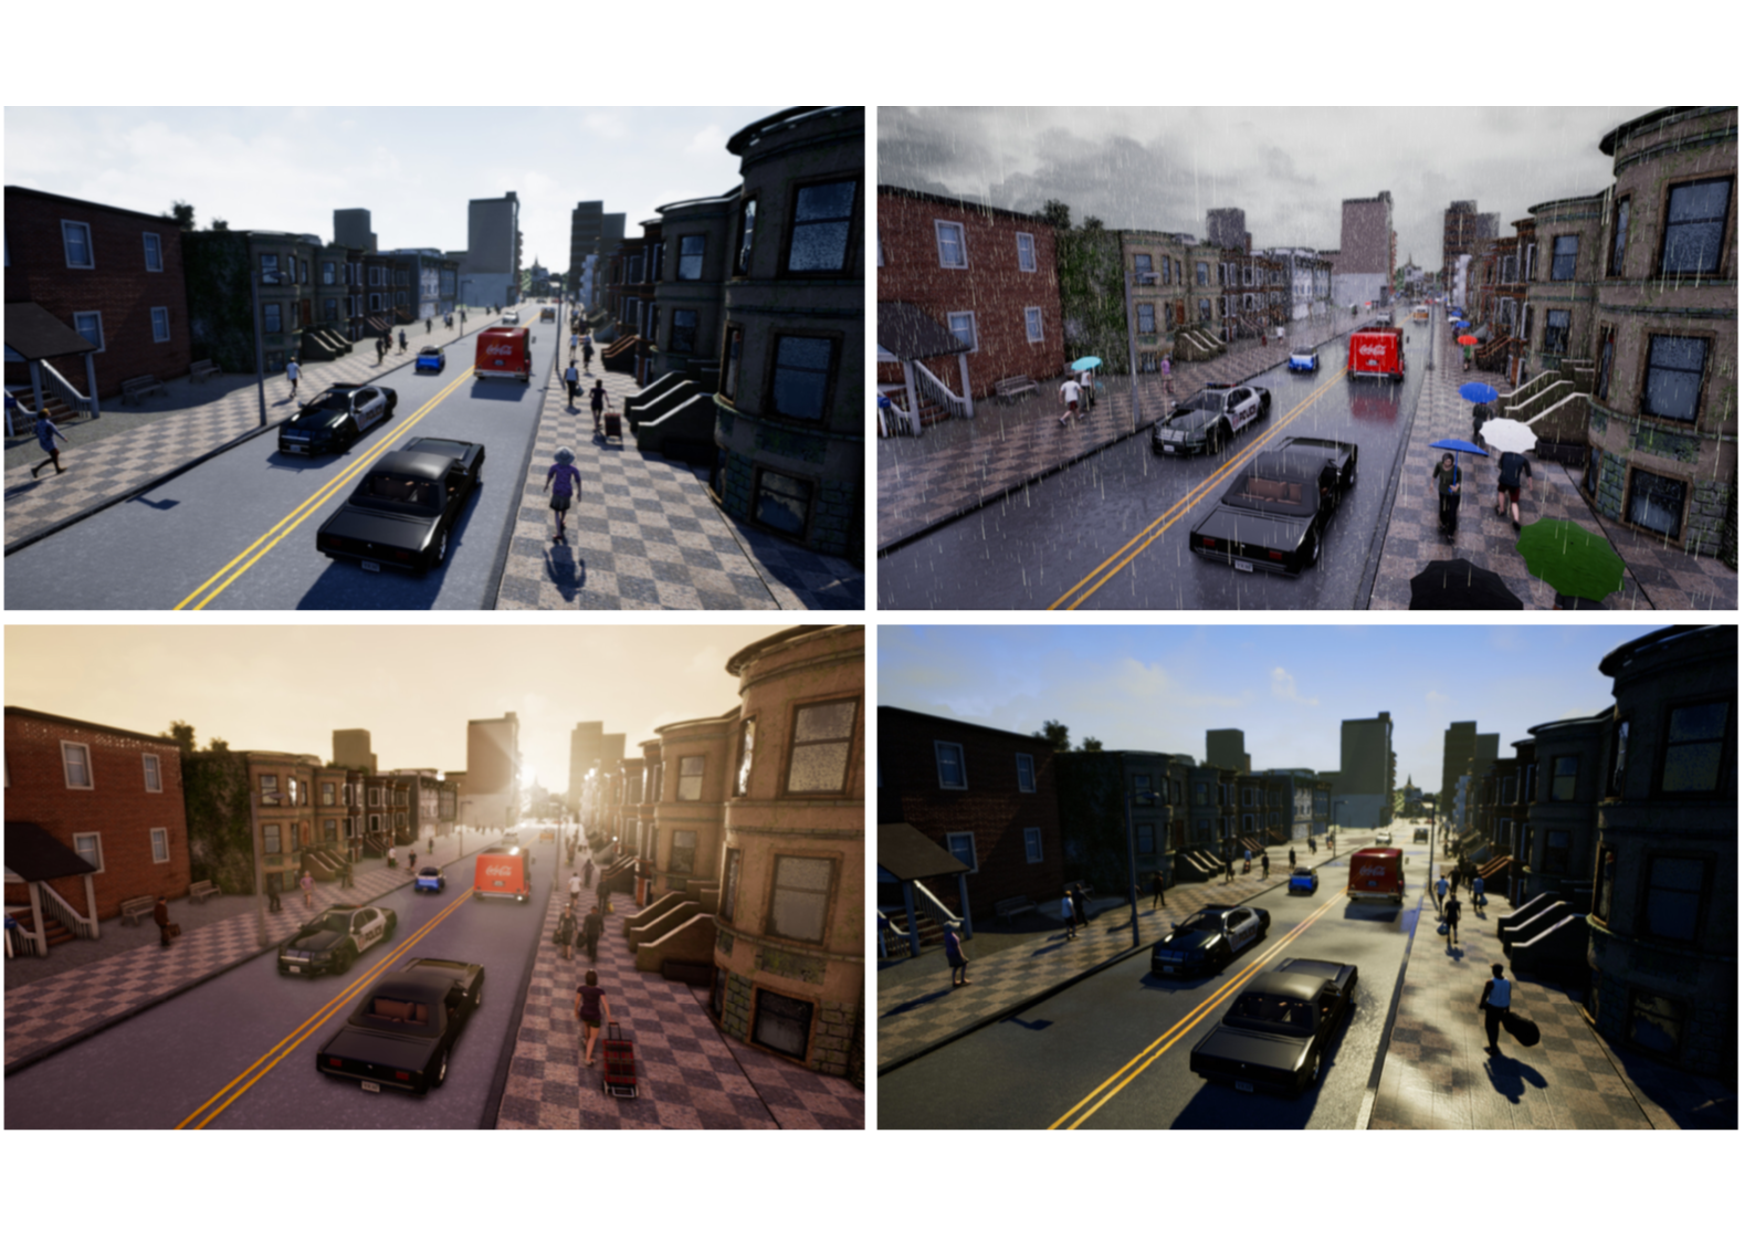
\includegraphics[width=12cm, height=5cm]{images/carlaWeather.pdf}
    \caption{Carla-Different Weather Conditions}
    \label{fig:weatherSituation}
\end{figure}
Carla developers believe that To make the simulation more similar to the real driving environment, different weather conditions i,e. rainy weather when the street is slippery for driving, or snowy, dark and fuggy weather should be also considered. In most of the presented simulation, weather situation has been neglected because developers mostly care about driving algorithms and maneuvering \acrshort{av} regardless of the environment where maneuver should be performed. Most of the images for detection parts are taken with the best camera quality but what if an \acrshort{av} confronts a situation like rainy weather where the street is more slippery than the environment it was trained or a dark weather when there is not enough light to take perfect photos for vehicle detection. So this was a smart idea from Carla developers to implement simulation in different weather environment.\\
Carla is implemented on UnrealEngine4(UE4) and its environments is a 3D environment which composed of static objects as building, street signs vegetation as well as dynamic objects like vehicles and pedestrians. The interesting point is that all of the accompanying assets which have been created by Unreal-Editor are released with Carla as open-source. In addition, Carla provides some sensors, pseudo-sensor readings and also a range of measurements associated with agent like the location and rotation of vehicle with respect to the world coordinate system. 
\subsection{Client-Server Sides}
Carla simulator is a client-server system. Server side runs and renders Carla world which includes simulation and scenes created by Unreal-Engine. Client side provides interface for users to interact with server like spawning new vehicles or controlling properties of simulation. Client \acrshort{api} is implemented in Python which is responsible for interaction between autonomous agent and server via sockets. Carla PythonAPI is a module that could be imported into python scripts which controls simulators and retrieve data like controlling vehicles or attach sensors into them and then reading data generated by sensors. Diagram \ref{fig:carlaModel} illustrates the client-server system in Carla.  
\begin{figure}
    \centering
    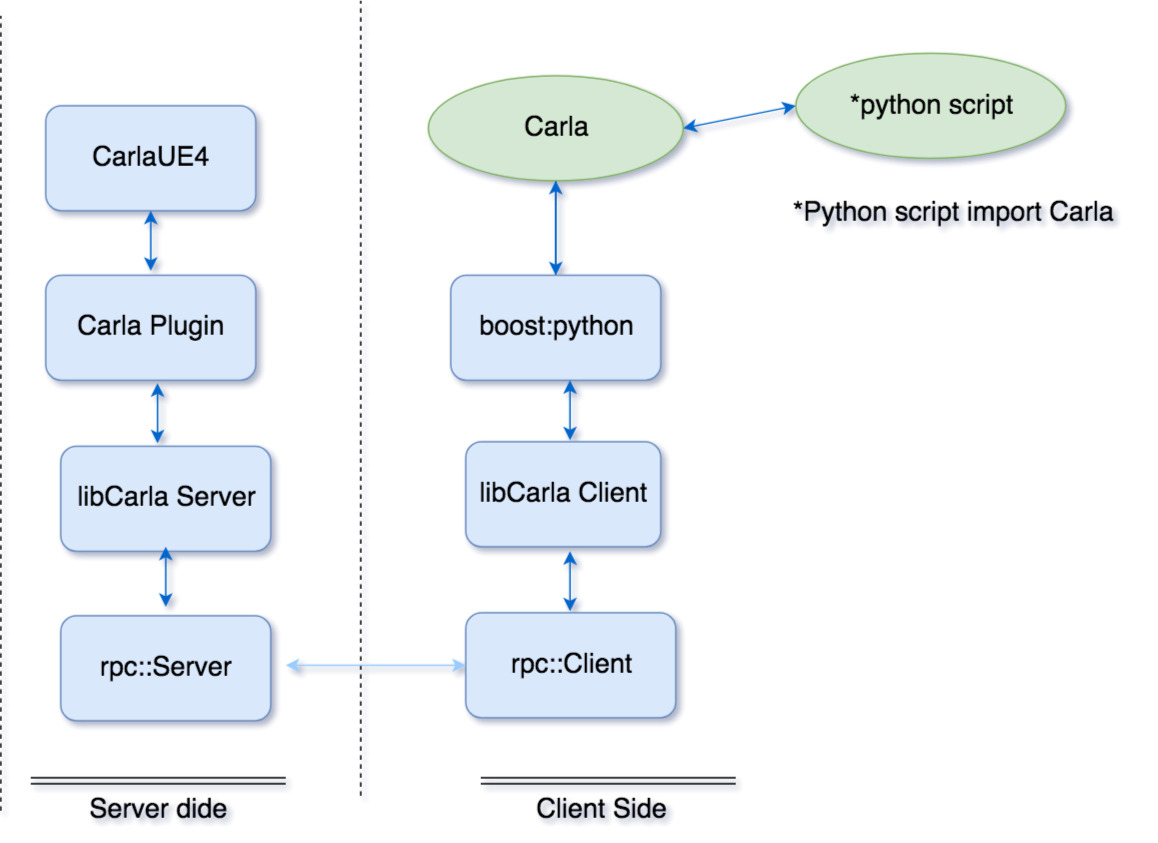
\includegraphics[width=12cm]{images/carlaModel.jpg}
    \caption{Client-Server system in Carla}
    \label{fig:carlaModel}
\end{figure}
\subsection{Sensors}
As explained above, Carla provides some sensors but this is still under-development. Here is a description of the Carla sensors which have been used during this work.
\subsubsection{Camera-Sensor}
This sensor was the first sensor presented by Carla developers which provides RGB cameras and pseudo-sensors. Pseudo-sensors presents ground-truth depth and semantic segmentation \cite{CarlaSimulator}. Sensor's parameters are 3D location, 3D orientation respecting to the vehicle coordinate, field of view and depth of field so it represents 3 modalities: normal vision, ground-truth depth and ground-truth semantic segmentation. Depth-camera or ground-truth depth provides a view which codifying the distance of each pixel to the camera. Semantic segmentation, classify objects in the scene as they will be presented in different colors. Segmentation is based on road, vehicles and building. Fig \ref{fig:segmentation} shows samples of different modalities in camera-sensor. In this work, we use camera sensor as a normal vision and it captures different photos during simulation. Results will be used for vehicle detection in our autonomous parking scenario.
\begin{figure}
    \centering
    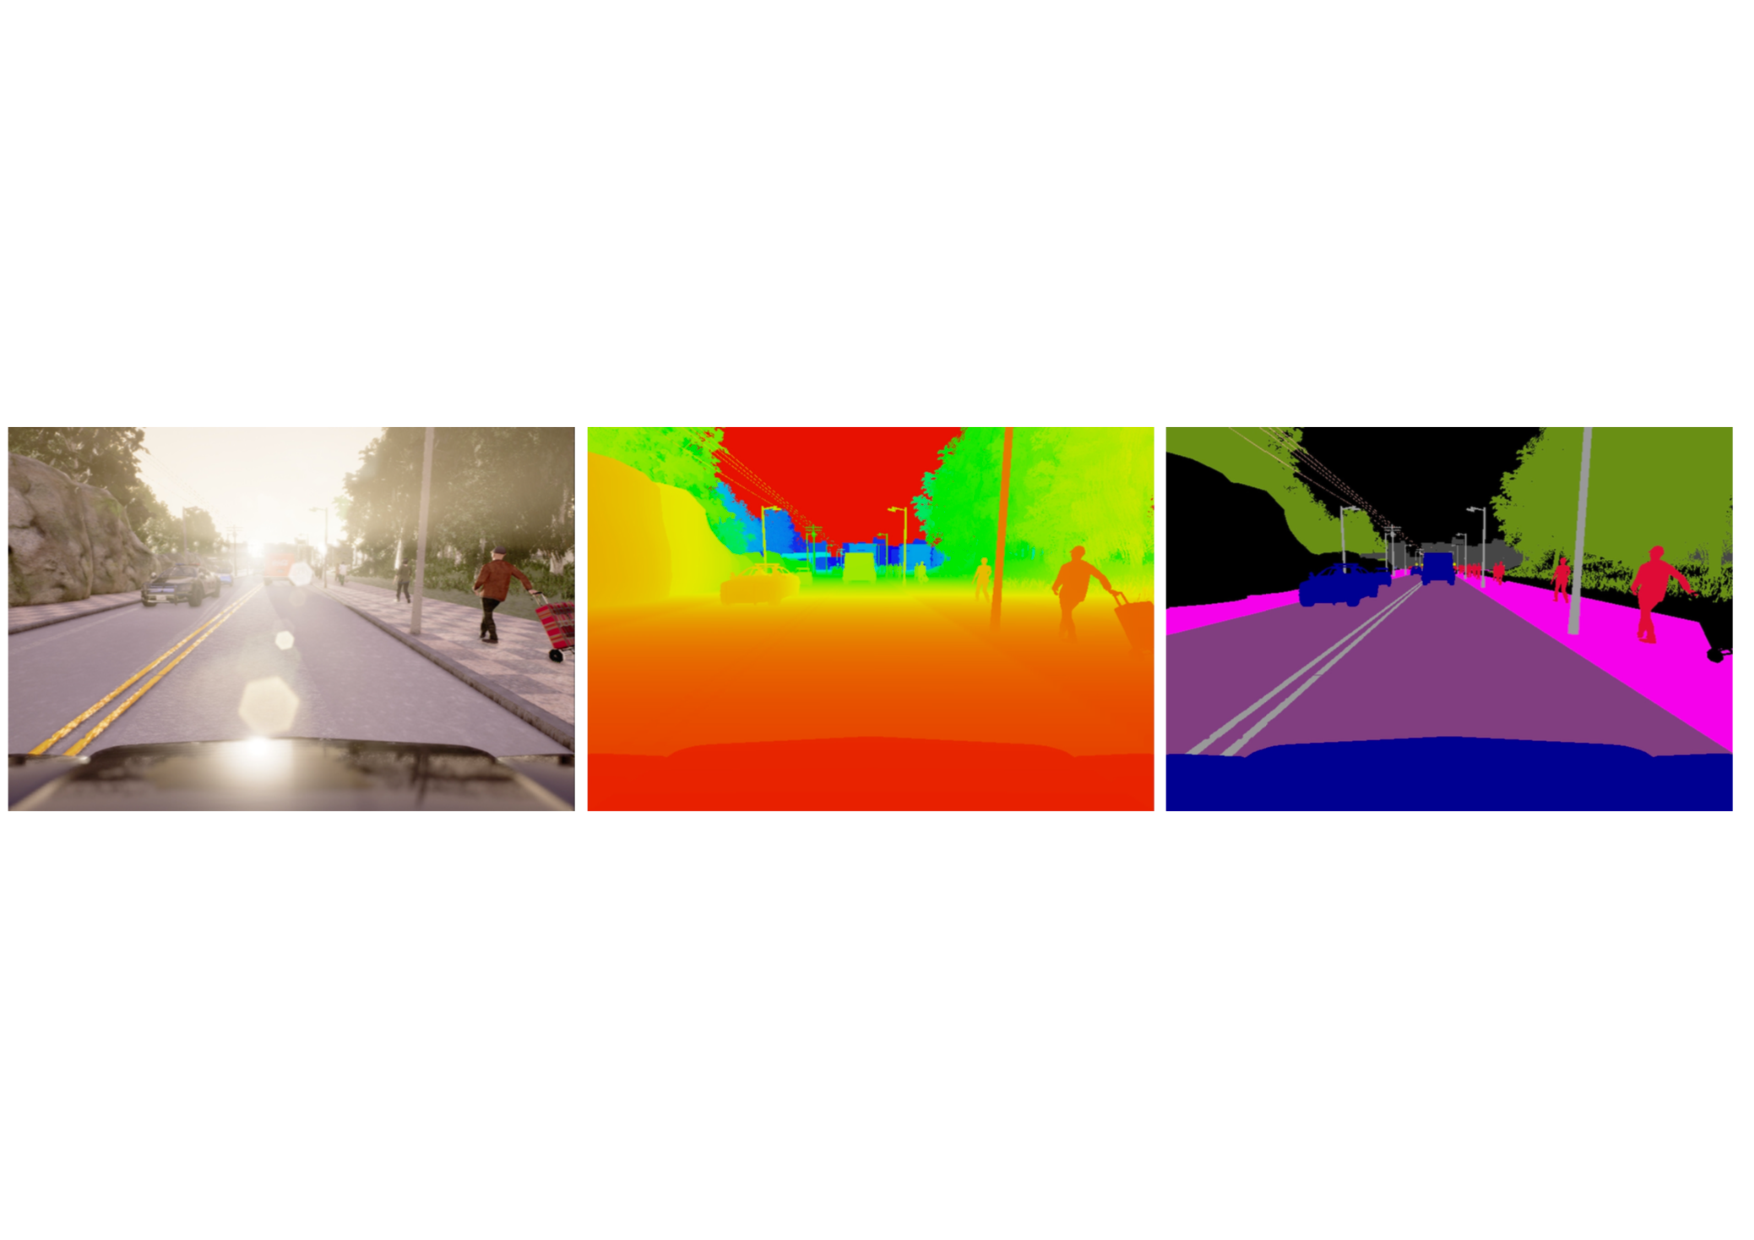
\includegraphics[width=12cm, height=6cm]{images/carla-segmentation.pdf}
    \caption{Carla-Camera Sensor Results}
    \label{fig:segmentation}
\end{figure}
\subsubsection{Gnss-Sensor}
\acrfull{gnss} sensor is attached to an actor to show its current position. This sensor is not considered as a detection sensor and does not provide any information of other vehicles or surrounding obstacles. However, it is sometimes useful to get the location of obstacles which are already detected. This location is Geo reference which defined by open-drive map definition.For example it shows longitude, latitude or altitude position of the actor. In this thesis, Gnss was used to help us finding the distance from the vehicle to the detected vehicle by attaching it to other vehicles. 
\subsubsection{Obstacle-Sensor}
This sensor detects other obstacles during simulation. Detection depends on the view and range of the sensor. This sensor is also supposed to provide distance to detected obstacle. However, this distance measurements have some problem yet.
\section{Common Concepts in Autonomous Parking}\label{concepts}
This section describes some of the expressions and concepts which has repeatedly been used in the next chapters.
\subsection{Ego Vehicle}
Ego-vehicle refers to the self-driving vehicle to which all of the driving algorithms(here parking maneuver) would be applied. Hence, ego-vehicle is our actor/agent that is connected to sensors and we want to monitor its behavior. In other words, when we talk about \acrlong{av}, we have to look beyond the first person's singular as developers call it ego-vehicle \cite{egoVehicle}.
\subsection{Non-Holonomic Vehicle}
The idea of our parking maneuver algorithm, is the vehicle is non-holonomic which means that there is no intolerable velocity constraint on vehicle \cite{parkingManeuver}. The idea of the parking maneuver method which have been used in this thesis, is to control a car based on its steering angle and velocity. In other word, it tries to turn vehicle's steering to reach to the expected point so there should not be any constraints on magnitudes of velocity and steering angle.
\begin{figure}
\centering
    \begin{tabular}{c|c|c}
         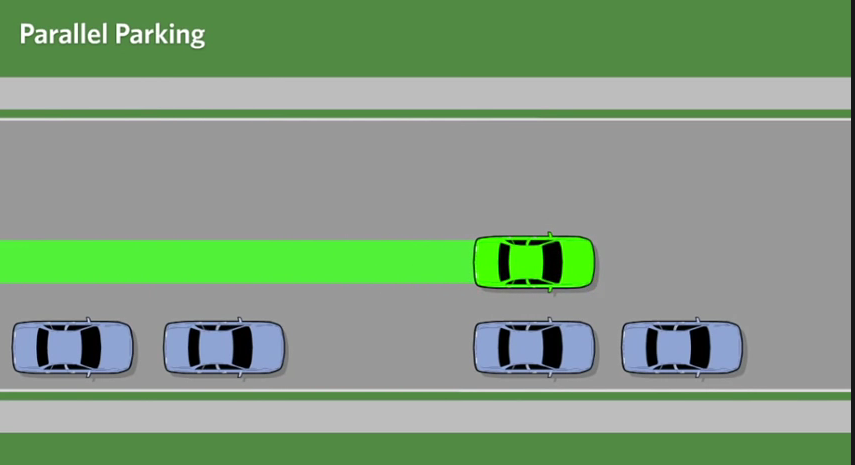
\includegraphics[width=4cm, height=4cm]{images/parallelParking.png} 
         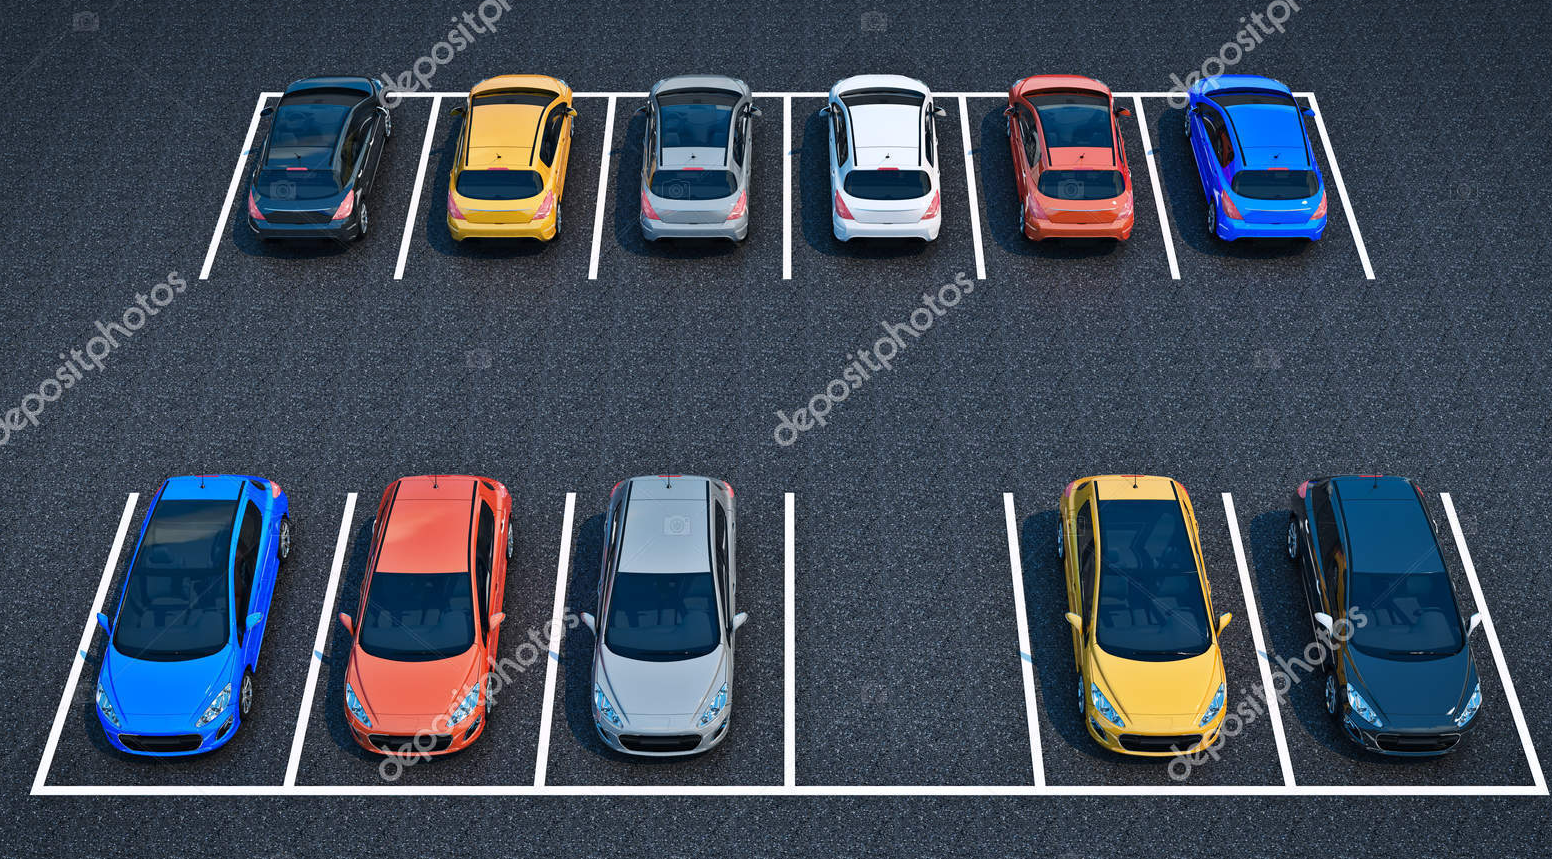
\includegraphics[width=4cm, height=4cm]{images/verticalParking.png}
         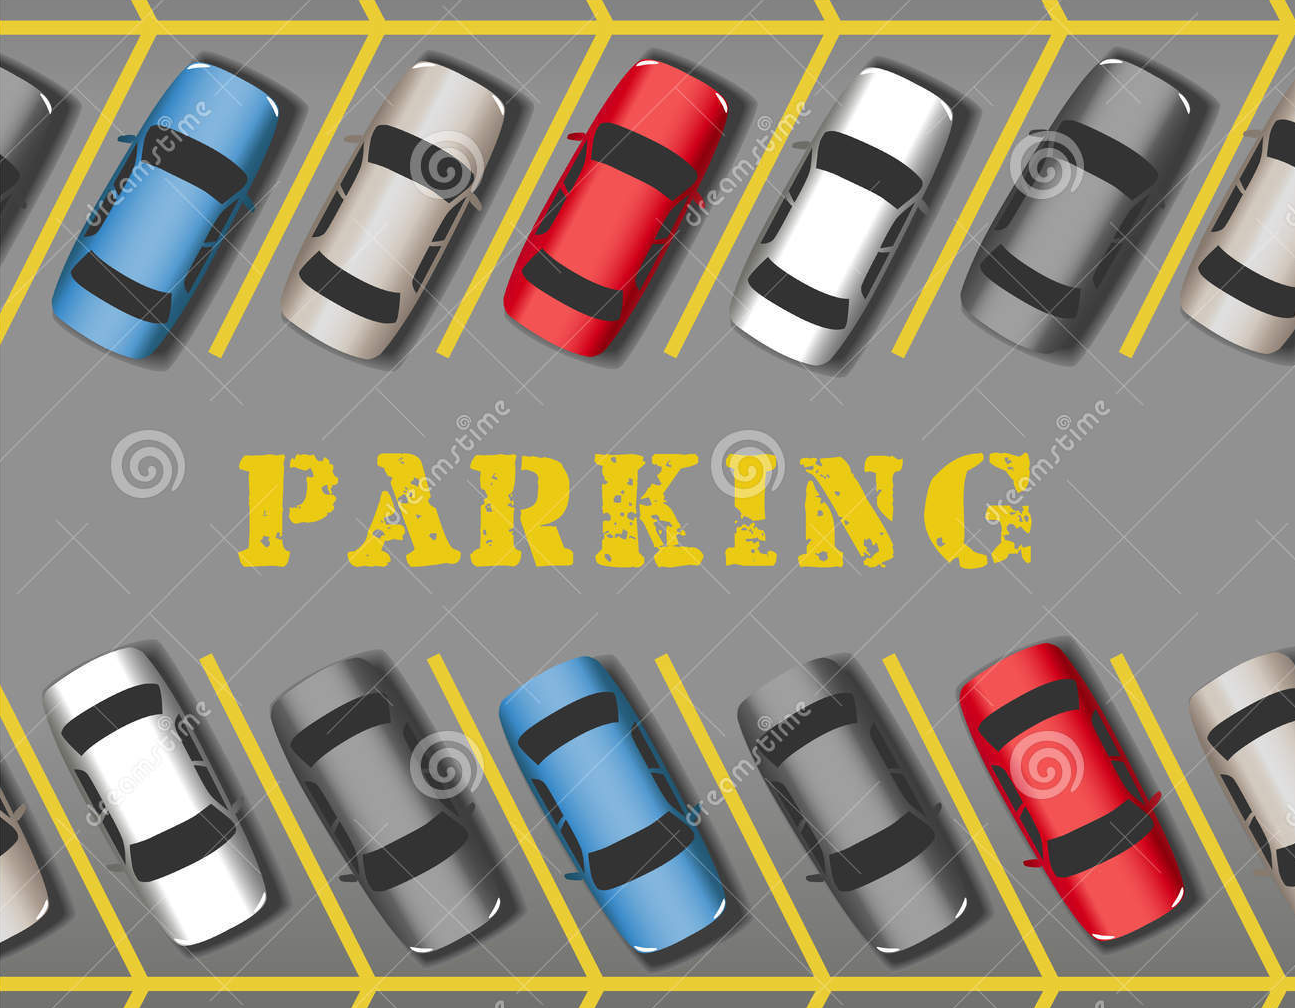
\includegraphics[width=4cm, height=4cm]{images/obParking.png}
    \end{tabular}
    \caption{Parallel Parking-Vertical Parking-Diagonal Parking}
    \label{fig:parkingTypes}
\end{figure}
\subsection{Parking Types}
There are three types of parking lots as it can be seen in \ref{fig:parkingTypes} \cite{novel-CLMR}
\begin{itemize}
    \item \textbf{Vertical Parking:} Vehicles should be parked in the boxes of a row which is vertical to the side of the parking place. This type is also called Perpendicular parking lot.
    \item \textbf{Diagonal Parking:} Diagonal parking is very similar to vertical parking but the separation lines of parking places(boxes) are diagonal.
    \item \textbf{Parallel Parking:} This parking lot can be seen on both sides of a street that that vehicles are in a row which are positioned parallel to each other. This thesis also works on this type of parking.
\end{itemize}
\section{Deep learning and machine learning} \label{ML}
\acrfull{dl} and \acrfull{ml} are fields of \acrfull{ai} while DL is a sub-field of ML. In both fields we study about design of an algorithm which could learn based on data we provided which are called training data. Hence, trained algorithm could present some results in the future without programming again based on what it has learned. There are three types of learning:\cite{AI}
\begin{itemize}
    \item \textbf{Supervised-Learning:} Training process is based on some labeled data as the labels says the algorithm what should be predicted.
    \item \textbf{Unsupervised-Learning:} There is no labeling or control during training process and the algorithm should find patterns in data. This learning type can be used in visualization and analysis process.
    \item \textbf{Reinforcement-Learning:} This method which contains an agent(robot) which is learned to behave in an environment by taking actions and quantifying results. Robot should takes next action based on the current state and gets reward for its correct decision so it will learn based on these rewards. This method has been used in play games like chess, traffics lights and other control systems.
\end{itemize}
Above learning methods are common in both \acrshort{dl} and \acrshort{ml}. However, DL is one way of executing \acrshort{ml}. \acrshort{dl} tries to make a deeper execution of \acrfull{nn}. As \acrshort{nn} is defined with three layers(fig \ref{fig:NN}). Deep learning adds multiple weights or hidden layers between input and output layers of shallow \acrshort{nn} to make it deeper \cite{AI}. One of the other difference between \acrshort{ml} and \acrshort{dl} is that \acrshort{ml} always needs a guidance to learn but \acrshort{dl} is better in classification learning so DL could learn on its own because it structures the algorithm in \acrshort{nn} layers in a way that could be learned and made decision. However, \acrshort{dl} needs lots of data, memory and time for learning as in some cases when there are many data, it would take months to finish learning process in \acrlong{dl}.
\begin{figure}
    \centering
    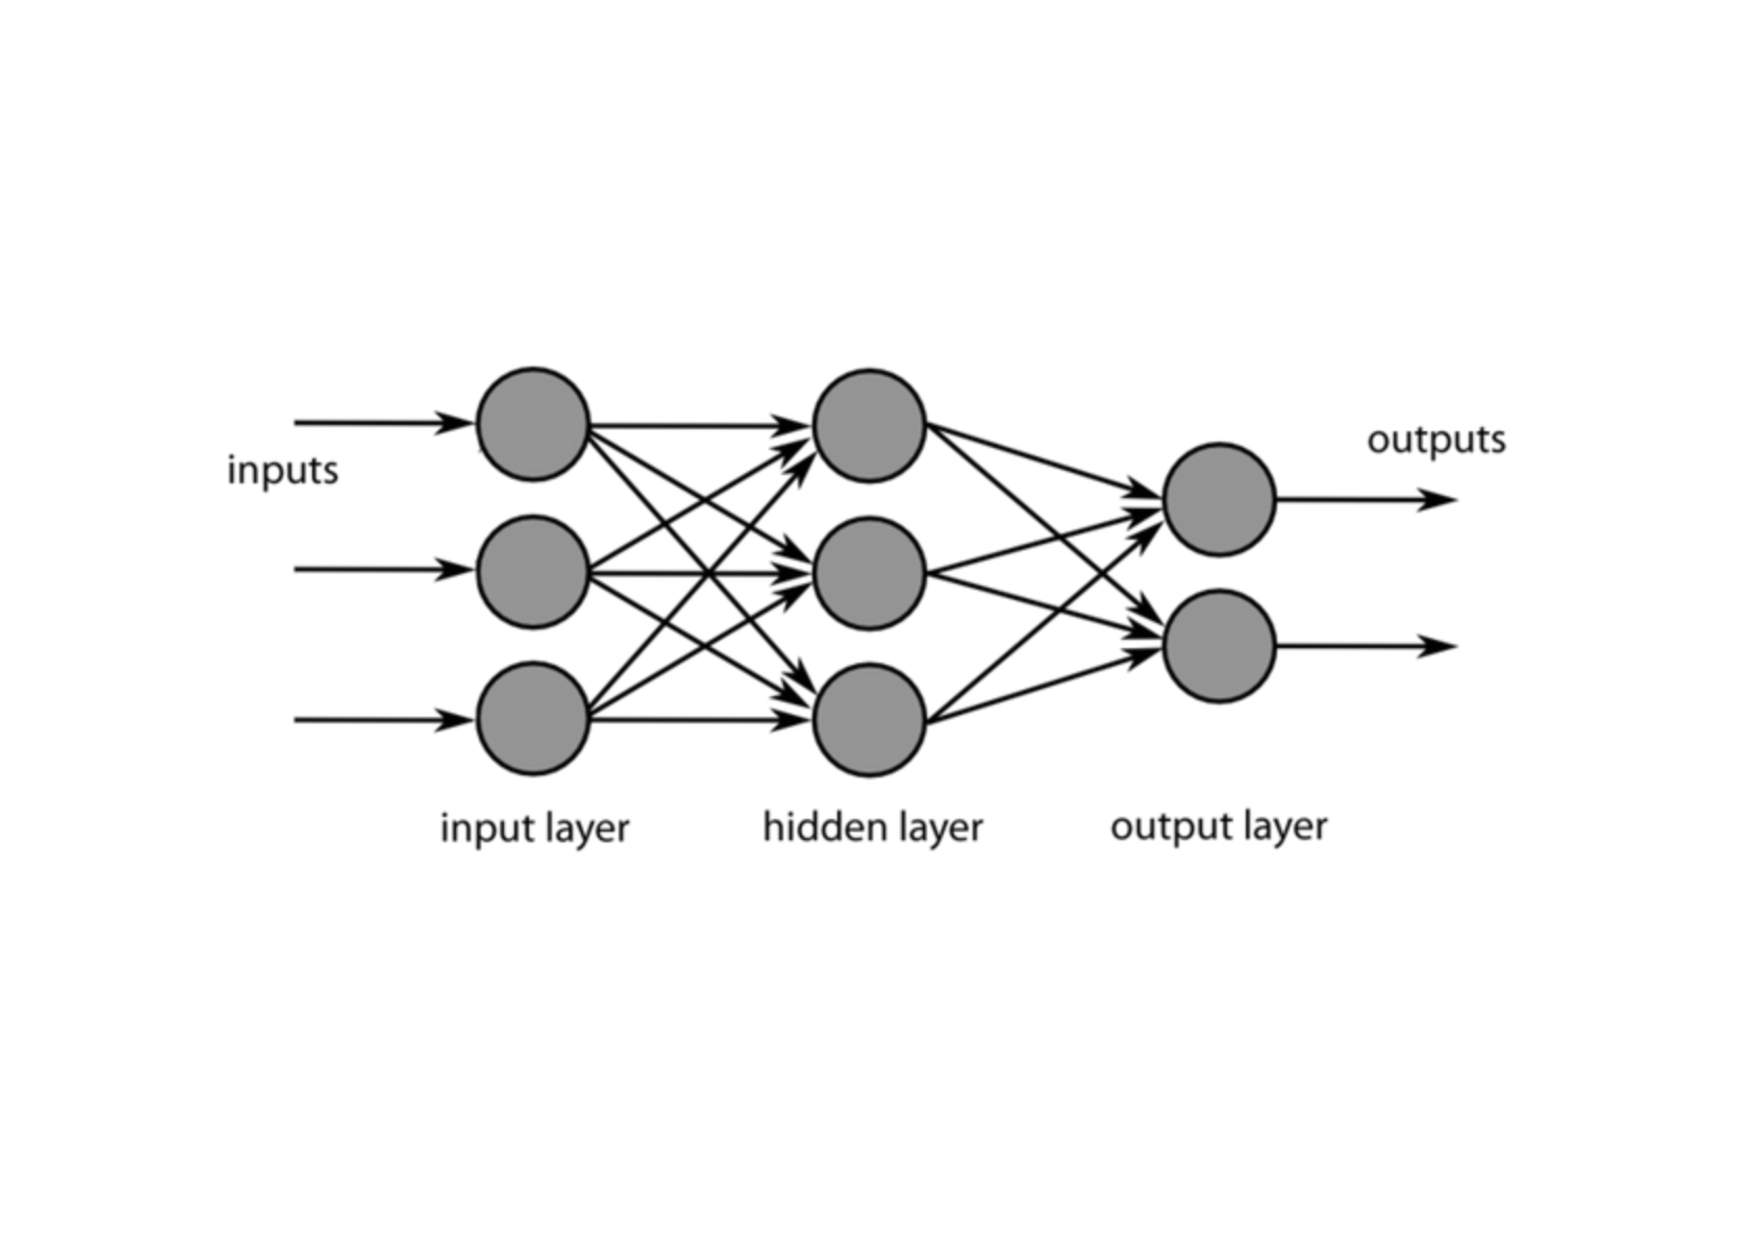
\includegraphics[width=12cm, height=6cm]{images/NN.pdf}
    \caption{Neural Network Layers}
    \label{fig:NN}
\end{figure}
\subsection{Object Detection Methods}
After reviewing the concepts of learning(\acrshort{ml} and \acrshort{dl}), here are some of the methods and algorithms for learning which are used in object detection. During this thesis two of these methods(Faster-RCNN and ACFObjectDetector) have been used for vehicle detection as it will be explained in chapter \ref{chapter:Parking Space Detection}.
\begin{itemize}
\item \textbf{\acrfull{hog}}-
 \acrshort{hog} is an old and popular method. Since it is not using a specific deep learning algorithm, it is a fast method. This simple method could not be handled to detect objects in different orientation or object rotation.
    \item \textbf{CNN:} \acrfull{cnn}s are similar to the human neural networks but they added some synapses(weights) so empowered \acrshort{nn} and complex dataset could be learned through the network \cite{CNN}.
    \item \textbf{\acrshort{rcnn}-FastRCNN-FasterRCNN:} \acrfull{rcnn} is region based \acrshort{cnn} and is a \acrshort{dl} method which adds some manageable number of regions into \acrshort{cnn} so it combines rectangular region proposals with CNN features. The process in \acrshort{rcnn} algorithm is as follows: \cite{RCNN-matlab}
    \begin{enumerate}
        \item Find regions in image that might contains objects which are called region proposals.
        \item Extract CNN features from the following regions.
        \item Classify objects by using extracted features.
    \end{enumerate}
    In order to speed up R-CNN, Fast-RCNN was introduced. Fast-RCNN uses an external edge boxes algorithm for generating regions and it is faster than R-CNN because its detector process the entire image instead of classifying each region and as FastRCNN contains computations for overlapping regions, that is more efficient than RCNN. And finally FasterRCNN is the fastest detection method because instead of using an external edge boxes algorithm(as in FastRCNN), it adds \acrfull{rpn} boxes directly to the network for generating regions. Fig \ref{fig:table} compares these methods \cite{RCNN-matlab}.
    \begin{figure}
        \centering
        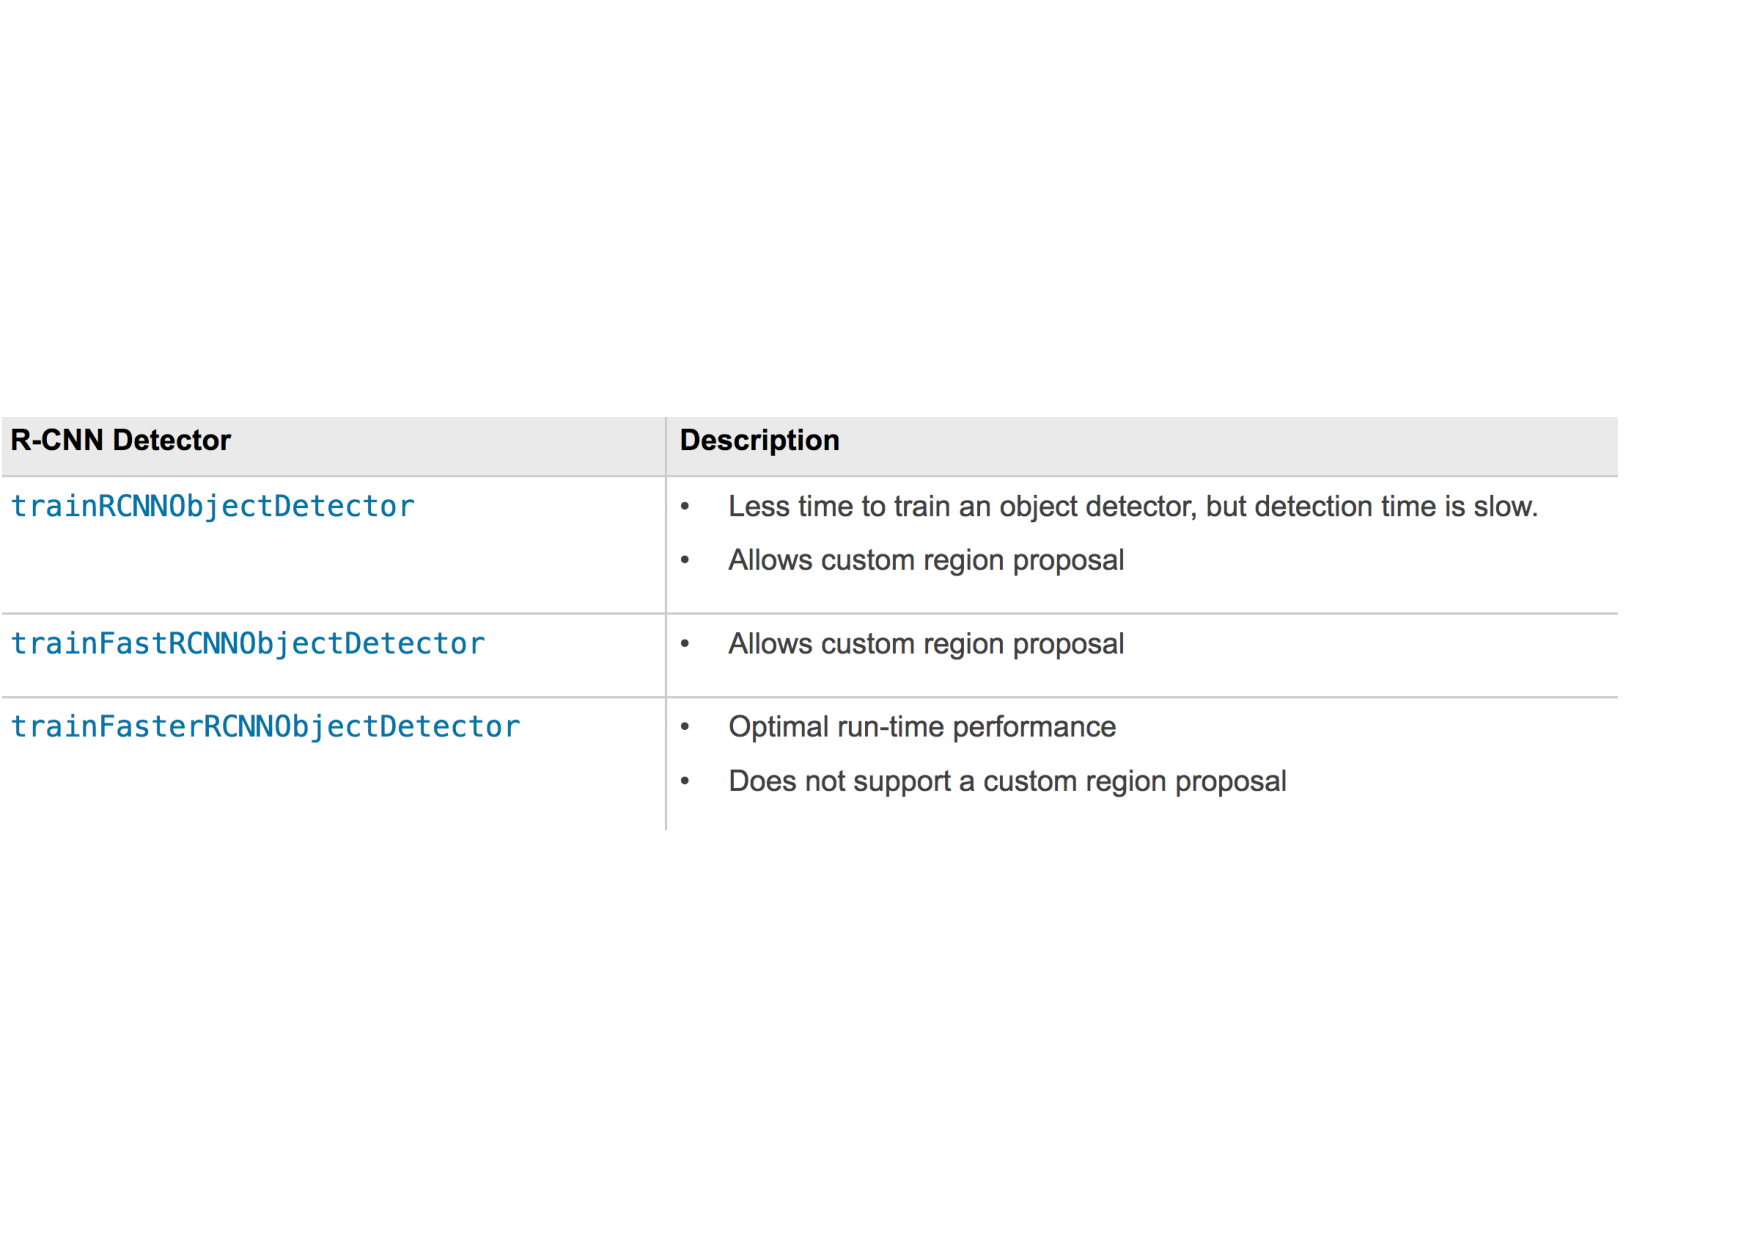
\includegraphics[width=12cm, height=6cm]{images/table.pdf}
        \caption{Comparison of \acrshort{cnn} Methods} 
        \label{fig:table}
    \end{figure}
    \item \textbf{MaskRCNN:}
    Recently a new method on FasterRCNN has been defined which is called Mask-RCNN \cite{MaskRCNN}. This method extends FasterRCNN by adding a branch for segmentation masks on each region of interests(ROI). It provides all of the outputs generated by FasterRCNN: class labels and bounding-boxes. Besides, Mask-RCNN adds an additional mask output which include pixel to pixel alignment of detected objects. Fig \ref{fig:maskRCNN} illustrates some results of MaskRCNN.
    \begin{figure}
    \centering
        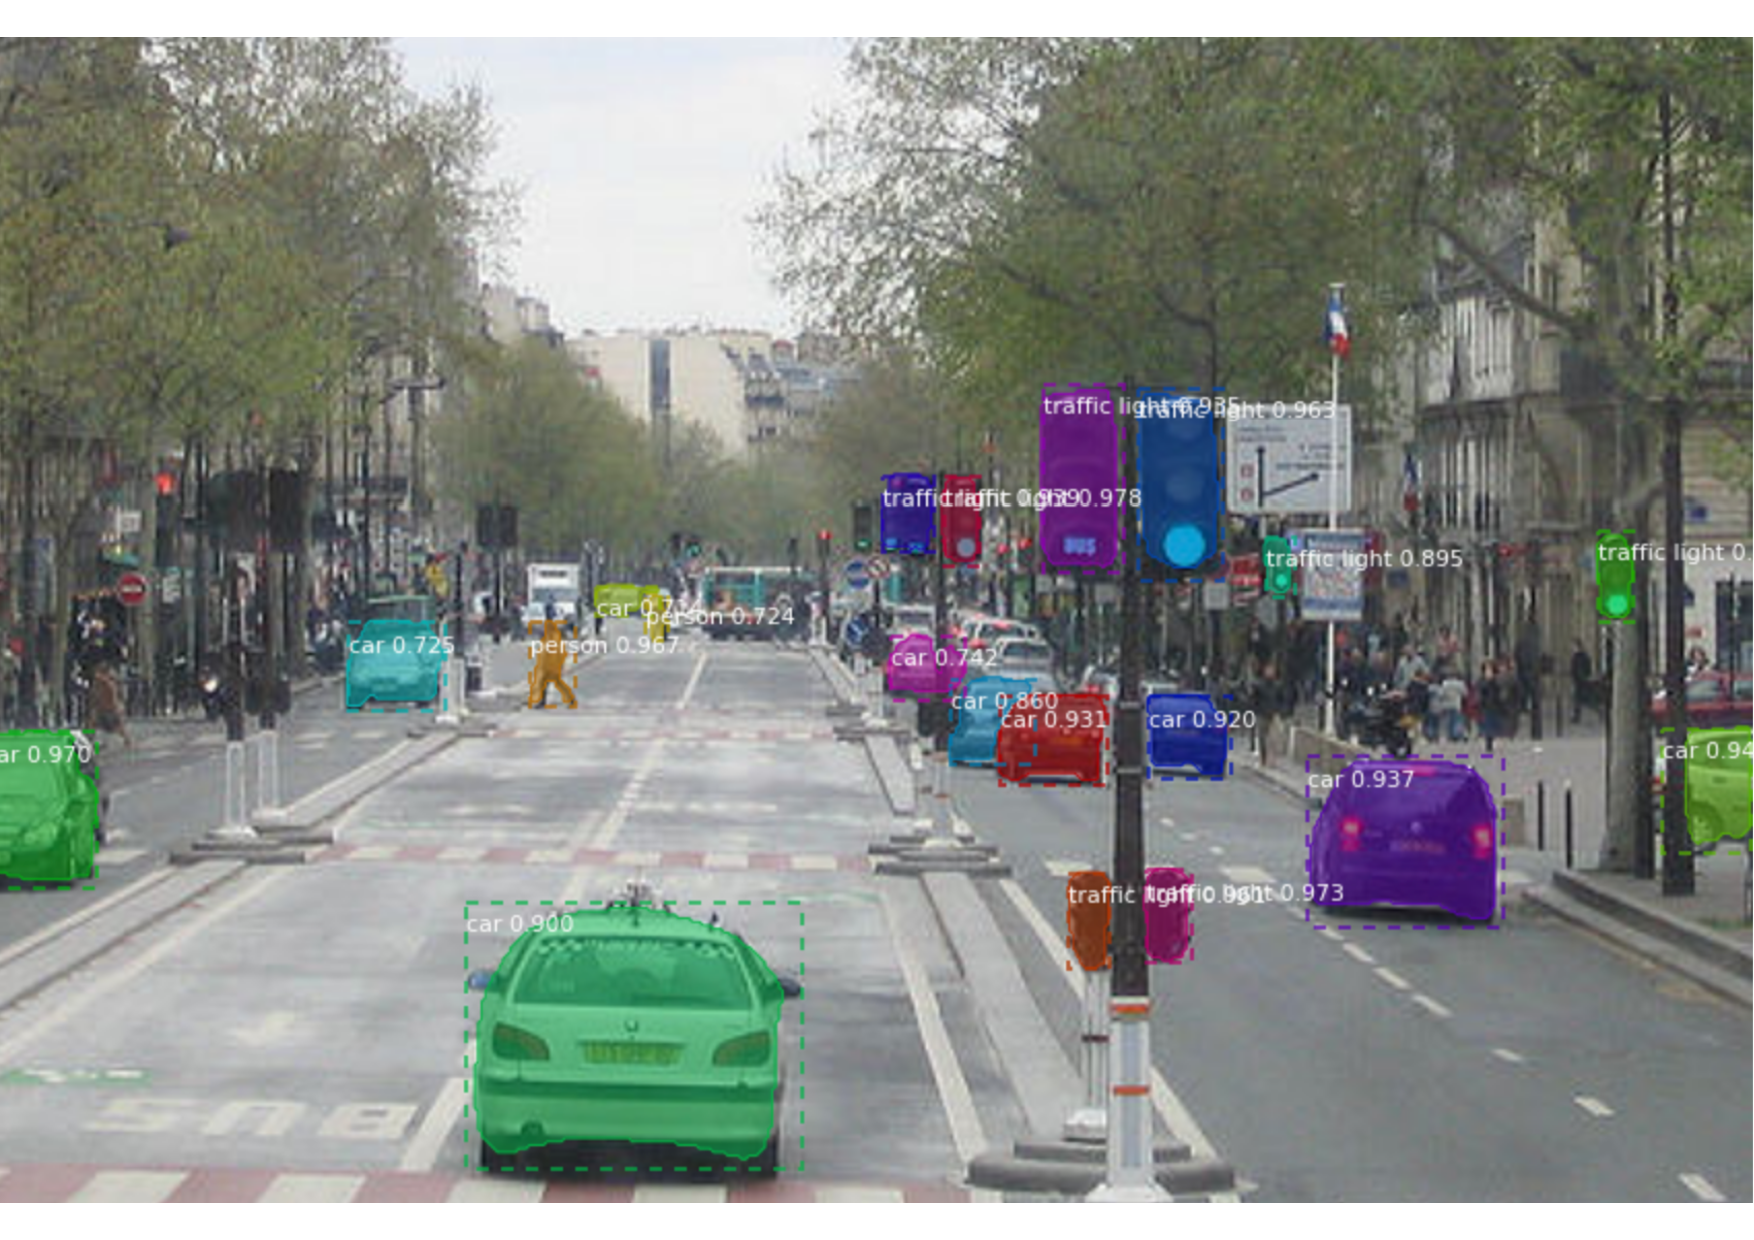
\includegraphics[width=12cm, height=8cm]{images/maskRCNN1.pdf} 
        \caption{Mask-RCNN}
        \label{fig:maskRCNN}
    \end{figure}
    \item \textbf{\acrfull{yolo}:} \acrshort{yolo} is another object detector in \acrlong{dl} Which is presented to provide a faster approach than other object detectors and even FasterRCNN. This method runs deep learning \acrshort{cnn} on an input image to produce network predictions. Then in the next step object detector decodes all predictions and generates bounding boxes.
    \item \textbf{ACFObjectDetector:} \acrfull{acf} is a simple method in object detection and its detection is based on object features. \acrfull{acf} recognizes specific objects based on training images and object ground truth locations \cite{ACF}. This method has been also selected for this work because after testing several methods, ACF presented better results in our data.
\end{itemize}


